\documentclass[12pt,a4paper]{article}

\usepackage[left=2cm, right=2cm, top=2cm, bottom=3cm]{geometry}

% Input encoding and typographical rules for English language
\usepackage[utf8]{inputenc}
\usepackage[english]{babel}
\usepackage[english]{isodate}

\usepackage{bytefield}
\usepackage{caption}
\usepackage{enumitem}
\usepackage{graphicx}
\usepackage{multicol}
\usepackage{times}

\makeatletter
\renewcommand{\maketitle}{
{\Huge\textbf{\@title}} \\
\noindent\rule{\textwidth}{1pt} \\
\medskip
}
\makeatother

% Section header size and spacing
\makeatletter
\renewcommand{\section}{%
  \@startsection{section}{1}{0pt}{-3.5ex plus -1ex minus -.2ex}{2.3ex plus .2ex}{\Large\bfseries\sffamily}%
}
\makeatother

% Removes paragraph indentation
\setlength{\parindent}{0pt}

% Configures the spacing between paragraphs
\setlength{\parskip}{12pt} 

% No numbering for section titles
\setcounter{secnumdepth}{0}

% Remove spacing between items
\setlist[itemize]{itemsep=0pt}

% ============================================================================ %

% These define global texts that are used in headers and titles.
\title{mea-craft}
\author{Felipe Paiva Alencar}
\date{June 2023}
% \revision{Revision 1}

\begin{document}
\maketitle

\begin{multicols}{2}

\section{Project Details}

\begin{itemize}
\item Author: Felipe Paiva Alencar
\item Subject: Embedded Systems - Pascal Benoit
\item University: Polytech Montpellier
\item Date: June 2023
\end{itemize}

\section{Features}

\begin{itemize}

\item \textbf{RISC-V Core:}
\begin{itemize}
\item DIY implementation of the RV32I instruction set architecture (ISA),
providing a flexible and customizable processing core.
\item Uses the AXI4-Lite memory interface enabling a seamless interface with
different memory devices.
\item Has support for interrupts allowing the implementation of event-driven
functionalities.
\end{itemize}

\item \textbf{Graphics:}
\begin{itemize}
\item The sprite architecture presented in class, has been enhanced to enable
dynamic changes to sprite contents, multiple texture scales, and memory sharing
between sprites.
\item Fully parametric, has support 80 sprites arranged in 5 clusters in the
default configuration.
\end{itemize}

\item \textbf{Memory:} 
\begin{itemize}
\item 4 kilobytes of ROM: Storing a small bootloader that also performs a quick
test of the ISA implementation.
\item 64 kilobytes of RAM: More than sufficient memory capacity to
handle game, texture, and world data.
\item 20.48 kilopixels of texture memory: arranged in 5 clusters of sprites.
\end{itemize}

\item \textbf{Peripherals:}
\begin{itemize}
\item General Purpose Input/Output (GPIO) that allows the interface of the
software with the buttons and switches. 
\item Universal asynchronous receiver-transmitter (UART) that provides a
communication channel.
\end{itemize}

\item \textbf{Build Tools:}
\begin{itemize}
\item The build and flashing process is efficiently automated by a well designed
Makefile, simplifying the compilation, texture packaging, world generation, and
linking tasks.
\item Support for bulding and flashing via a single command, saving valuable
development time and effort.
\end{itemize}

\end{itemize}
\end{multicols}

\pagebreak

\section{Hardware}

\begin{center}
\captionof{figure}{Top Architecture}
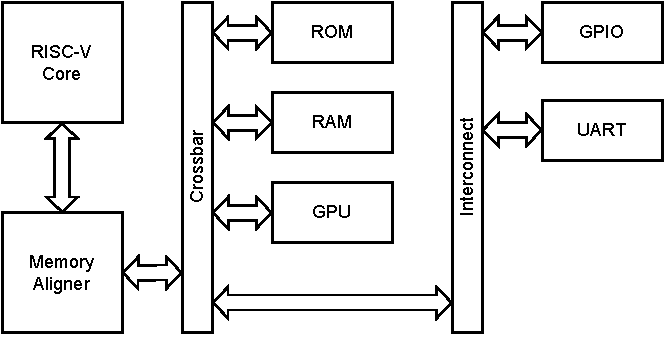
\includegraphics{schema0.pdf}
\label{fig:schema0}
\end{center}

The top architecture is composed of a RISC-V core, a memory aligner, a crossbar,
read-only memory (ROM), random-access memory (RAM) and simple 2D graphics
accelerator. Futhermore, the GPIO and UART are classified as peripherals and
communitate with the CPU via a simpler interconnect.

Everything is interconnected with the help AXI4-Lite interfaces. The crossbar
and interconnect are imported from the \texttt{verilog-axi} library.
Everything else, including the RISC-V core, was completely developed in-house.
Both of them are overkill for this context, but this architecture was conceived
with the use of multiple cores in mind where the use of crossbars and
interconnects would be fundamental.

The RISC-V core implements the \texttt{rv32i} Base Integer Instruction Set. The 
\texttt{Zicsr} Control and Status Register (CSR) Instructions were also
implemented because they are essential for the implementation of interupts. 
Interrupts were implemented, but are not currently used for anything useful.
The core is multicycle but not pipelined. A simple ISA test is performed by the
bootloader in order to maintain one's mental well-being during the process of
software development.

The read-only memory (ROM) is 4 kilobytes long and is used by bootloader. The
use of a bootloader developed to avoid having to rebuild the FPGA bitstream 
every software iteration.

The random-access memory (RAM) is 64 kilobytes long and is used for the C code,
texture data and world data. The texture data is initially located in RAM, but
is moved to the video memory before the start of the game. This allows for 
changes in the textures without having to rebuild the bitstream. In fact, one
could implement a completely different game without rebuilding the hardware 
implementation.

The General Purpose Input/Output (GPIO) implementation is very basic consisting
of simple registers. Therefore, there is no hardware support for changing the 
GPIO state with a mask.

The Universal Asynchronous Receiver Transmitter (UART) operates at 115200 bauds
with 8 data bits, 1 stop bit and no parity bits. This interface is fundamental
for the bootloader and is very helpful during software development since it
provides some kind debuging support through the use of the \texttt{printf}
function.

\begin{center}
\captionof{figure}{GPU Architecture}
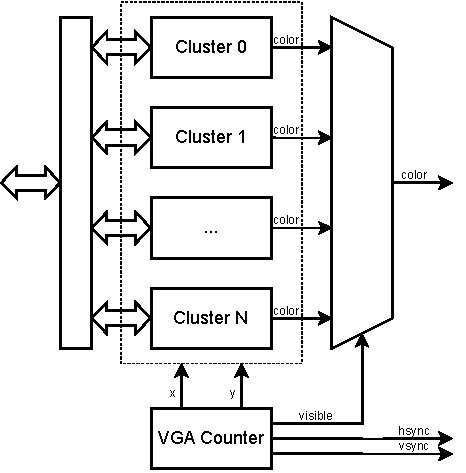
\includegraphics{schema1.pdf}
\label{fig:schema1}
\end{center} 

The graphics accelerator developed in class was greatilly overhauled into the
architecture described in the schema above. The renewed architecture is fully
parametric and is capable of displaying 80 sprites with transparency support 
in the current configuration. These sprites are divided in 5 clusters. 
A cluster is a group of sprites that uses the same texture RAM. This division
was introduced to mitigate the hardware size. A perk of this architecture is
that transparency does not work between overlapping sprites in the same cluster.
Futhermore, a sprite is not obliged to use the whole texture. A sub-region can
be configured for each sprite through register access in software.

The GPU has AXI4-Lite interface that allows for cluster register access. This
interface is not propaged to the clusters because it's features are not needed
and using a simpler interface reduces hardware complexity. Therefore, a 
converter is present in the GPU top architecture. The converter is not present
in the schema.

The VGA Counter provides the VGA synchrony signals and the current position of
the electron beam in the screen. This position is used by each cluster to
compute the pixel color value. Finally, combinatory logic decides the final
value of the VGA color signals based upon the color value of each cluster,
the visibility signal of the VGA Counter and the cluster priority order. 
Transparency is implemented resignifying the value 0xFFF to mean transparency.
The sky color is hardcoded in this logic.

\begin{center}
\captionof{figure}{Cluster Architecture}
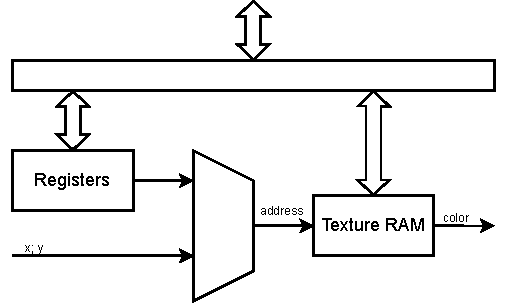
\includegraphics{schema2.pdf}
\label{fig:schema2}
\end{center}

Each cluster is composed of registers that store the position and texture
coordinates of each sprite. With the position value, combinatory logic
computes the address that stores the current color value. Then, this value is
retrived in the texture RAM. A very simple interconnect provides a write-only
interface for the registers and RAM.

\section{Software}

In this case, a final project of the embedded systems subject, I belive that the
tools used to build the software (the game) are more relevant than the game it
self. Therefore, much thought and time were put into these tools.

I choose the Clang/LLVM toolchain due to its inherent focus on extensibility.
By utilizing this toolchain, I could, for example, seamlessly integrate my own
instructions into the assembler. However, it's important to note that no custom
instructions have been implemented thus far.

The \texttt{make} tool is extensively used to automate the building process,
determining the source code files that require recompilation and specifying how
they should be compiled. It accomplishes this by leveraging a set of rules and
dependency relationships defined in the \texttt{Makefile}. However, as an
experienced programmer, I have encountered more flawed examples of
\texttt{Makefiles} than commendable ones. Despite its imperfections, I have
invested considerable thought and consideration into this project's
\texttt{Makefile}. Additionally, I have integrated a few helpful scripts into
the build process. For instance, you can effortlessly execute
\texttt{make flash} to compile all textures, generate the world, compile the
code, link everything, and flash the resuting binary.

Moving on to the code itself, let's delve into how the interface with the
hardware is implemented. It's important to emphasize that, in this
architecture, the specialized is essentially just a region of memory for the
CPU. To handle this, the \texttt{hardware.h} header contains a set of 
definitions that abstract the memory mapping.

Among the \texttt{\#defines}, you will find \texttt{structs} that provide
information regarding how data is organized in the different hardware registers.
Additionally, there are further \texttt{\#defines} that enable the conversion
of pure addresses into pointers to these specialized
structures.

The usage of the \texttt{volatile} qualifier is crucial in this context. It
signals to the compiler that the associated variables may undergo unexpected
changes. By doing so, it prevents unwanted optimizations that could potentially
result in incorrect program behavior.

Ultimately, a robust and intuitive interface to the hardware is achieved,
which greatly facilitates software development and minimizes the risk of bugs.

\end{document}


